The goal of this project is to implement Maximin Affinity Learning of Image
Segmentation (or MALIS for short) as introduced in~\cite{turaga_maximin_2009}.
It is a method used to obtain an image segmentation that is mainly used on medical
imagery.\\

\begin{figure}[!htbp]
	\centering
	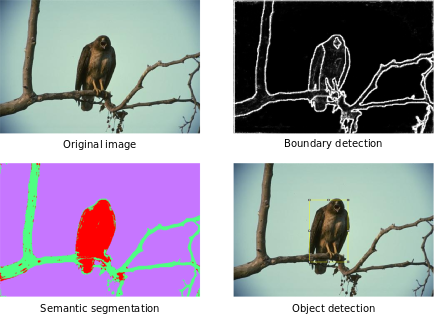
\includegraphics[width=0.7\linewidth]{./images/segmentation.png}
	\caption{Illustration of image segmentation, from
	\href{imagej.net/File:TWS-application-examples.png}{ImageJ}}%
	\label{fig:segmentation}
\end{figure}

As we can see in figure~\ref{fig:segmentation} there are multiple ways to
produce an image segmentation. In the top right corner we can see a boundary
detection of the original image, where borders between objects are in white and
objects are in black. Here we only get the separation between objects but no
information on the objects/segments themselves.\\
In the bottom left corner, we have an example of semantic segmentation of our
image. Here the idea is to classify every pixels in predefined classes (here
red is the bird, green the tree and purple the background). We then obtain a
segmentation with different information, which is not necessarily better than
boundary detection since both solve different problems.\\
On the bottom right corner we have an example of object detection. Even though
it gives us a rough estimate of the structure of the image and the objects
present in it, it is not considered  a segmentation and is a whole other class
of algorithms.\\

In the case of MALIS, we will try to obtain a boundary detection, or what we
could call an edge based segmentation. There are various ways to generate an
image segmentation of this kind, the simplest one being an algorihm such as
Canny's algorithm, or more advanced methods such as watersheds or more recently
neural networks based approaches. The idea with MALIS is to optimize directly a
measure of segmentation quality, which had not been done before. This is a
really interesting idea since segmentations are always evaluated using various
metrics (Rand Index, Variation Of Information ...) and optimizing one directly
could lead to better results, at least for this metric.\\

Our goal in this project is to implement the original MALIS
paper~\cite{turaga_maximin_2009} and also it's improvement
in~\cite{funke_large_2019}.\\

In this report, we will first describe how MALIS works in more details. We will
then look at how we implemented it and some implementation challenges that we
faced. We will then look at the results we have gotten so far, by implementing
the original method. Afterwards, we will look at how the method was improved
and what we will try to implement in the coming semester. Finally we will take
a look at how we worked as a team throughout this project.

